%%
%%
%% This file should be edited by user
%%

\chapter{bigAVR6} \label{chapter:bigAVR6}


\section{The Hardware}

This developmentboard, as shown in figure ~\ref{fig:bigavr6}, is produced by mikroElektronika and supports 64- and 100-pin AVR TQFP packages.

\subsection{Onboard - Features}

\begin{itemize}
 \item 2 x UART
 \item highspeed CAN transceiver MCP2551
 \item USB 2.0
 \item MMC/SD card slot
 \item digital thermometer DS1820
 \item onboard USB 2.0 programmer
 \item real-time clock DS1307
 \item 86 LEDs to indicate logic state of all microcontroller-pins
 \item 86 push buttons to control microcontroller digital inputs
 \item IDC10 connectors for all microcontroller pins
 \item DIP - switches to separate port pins from pull-up/down resistors
 \item potentiometer for testing the ADC - channels
 \item 1KBit serial EEPROM 24AA01
\end{itemize}

\subsection{Extensions}

\begin{itemize}
 \item 2x16 LCD, directly connectable via on-boad connectors
 \item 64x128 GLCD, directly connectable via on-boad connectors
 \item IEEE802.3 extensionboard 10MBit
 \item SmartMP3 decoder board
\end{itemize}


\begin{figure}[h]
 \centerline{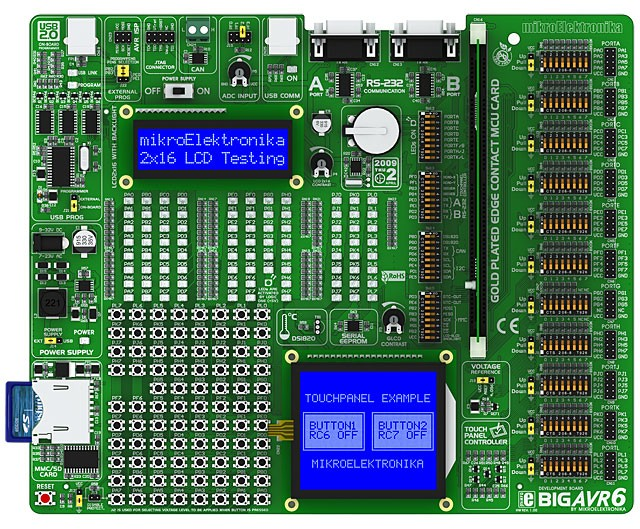
\includegraphics[width=.5\columnwidth]{pics/bigavr6.png}}
  \caption{bigAVR6 platform}
  \label{fig:bigavr6}
\end{figure}


\section{Supported Modules}

\subsection{GLCD}

The GLCD - extension consists of a KS0108B GLCD dot matrix liquid cristal graphic display system with a resolution is 128 x 64 pixel. As the schematics shows in figure~\ref{fig:glcd}, SW15/8 must be turned on to activate the GLCD-backlight, the contrast can be changed with potentiometer P3.

The GLCD is combined with a touchscreen foil, sticked onto the GLCD-surface. Activate SW13/1,2,3,4 to use it. To read the x and y coordinates, the component uses ADC channels 0 and 1, respectivly. 

The logic level of the following pins \textbf{MUST NOT} be touched by the programmer when using the GLCD and the touchscreen:

\begin{itemize}
 \item PORT A: 					all ports reserved for GLCD
 \item PORT E: PE2, PE3, PE4, PE5, PE6, PE7	reserved for GLCD
 \item PORT F: PF0, PF1 			reserved for touchscreen
 \item PORT G: PG3, PG4				reserved for touchscreen
\end{itemize}


\begin{figure}[h]
 \centerline{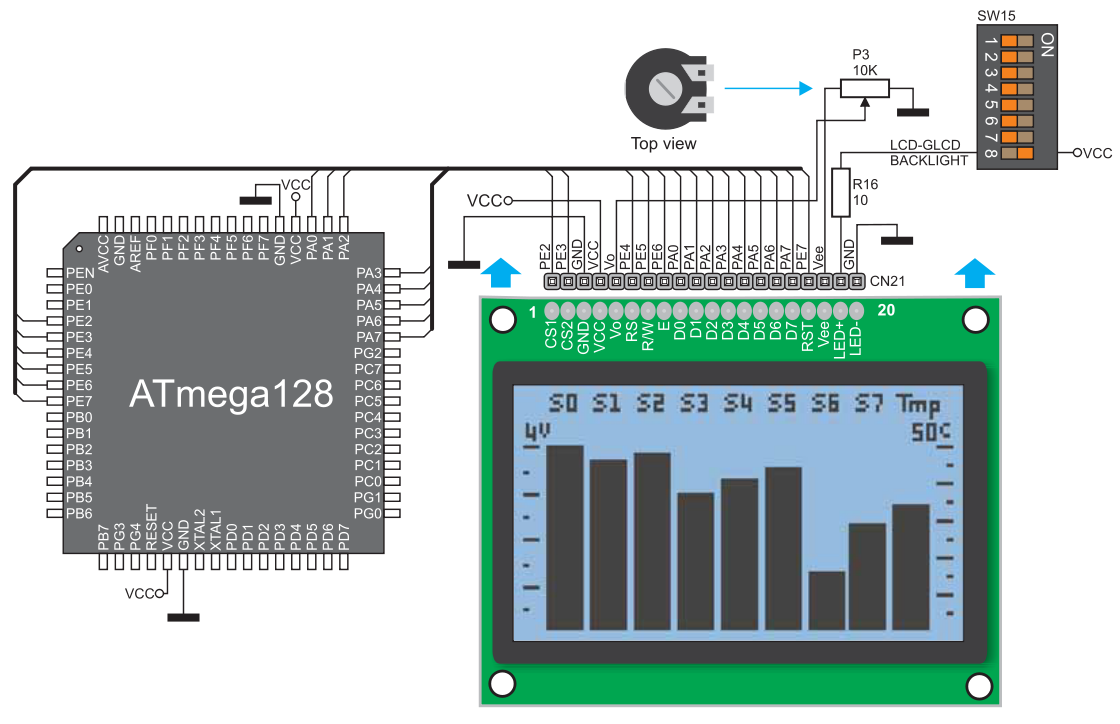
\includegraphics[width=.8\columnwidth]{pics/GLCD.png}}
  \caption{GLCD schematics}
  \label{fig:glcd}
\end{figure}

To use the GLCD in an application, component \textit{GLCDC} with interface \textit{GLCD} must be used. This interface provides functions for initializing, clearing, writing strings, and drawing graphical objects on the the GLCD. Additionally, it provides functions for calibrating the touchscreen and for getting x/y - coordinates. See listing \ref{GLCD} for all the provided functions. Figure \ref{fig:glcdc} shows the internal composition of the GLCDC: LCD128x64C is responsible for writing and initializing the GLCD, while TouchScreenC provides functionality related to determining the pressed positions. Therefore, TouchScreenC uses the parameterized interface Read\textless uint16\_t\textgreater wired to component AdcReadClientC for getting the needed ADC - values from channels 0 and 1.

\lstinputlisting[caption={GLCD.nc},label=GLCD]{../tinyos/tos/platforms/bigAVR6/GLCD/GLCD.nc}

\begin{figure}[h]
 \centerline{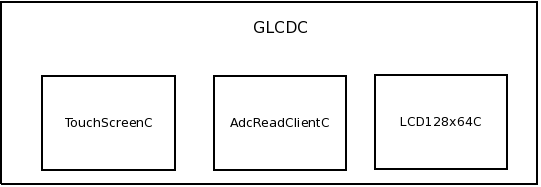
\includegraphics[width=.8\columnwidth]{pics/GLCDC.png}}
  \caption{GLCDC components}
  \label{fig:glcdc}
\end{figure}


\subsection{MMC}

A MMC/SD connector is available onboard so that memory cards can be interfaced to the microcontroller via SPI. As shown in figure \ref{fig:mmc}, activate SW15/3/4/5/6/7 to use it. Because the memory card is powered with 3.3V, whereas the microcontroller needs 5V supply, a 74LVCC3245 bus transceiver is used to obtain the needed voltage levels.

The logic level of the following pins \textbf{MUST NOT} be touched by the programmer when using the MMC:

\begin{itemize}
 \item PORT B: PB1, PB2, PB3			reserved for MMC: SCK / MISO / MOSI
 \item PORT G: PG1, PG2				reserved for MMC: CS / CD
\end{itemize}

\begin{figure}[h]
 \centerline{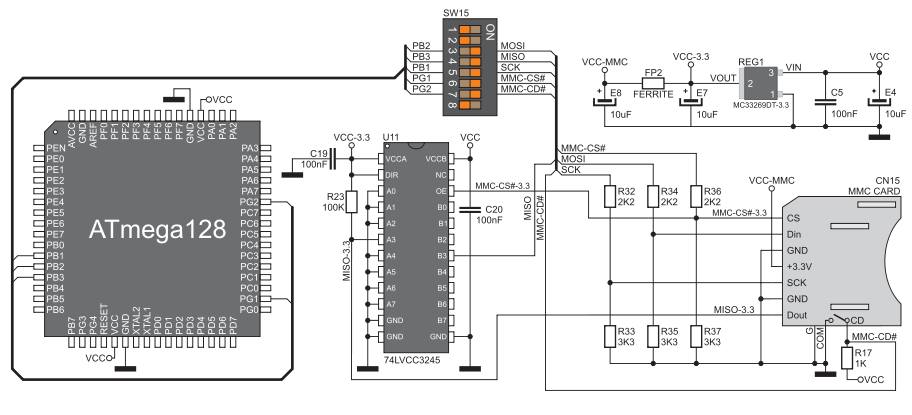
\includegraphics[width=.8\columnwidth]{pics/mmc.png}}
  \caption{MMC/SD Schematics}
  \label{fig:mmc}
\end{figure}

Component \textit{MMCC} provides interface \textit{MMC} to enable an application programmer to easily read \textbf{RAW} - data from a MMC, no write functionality is supported yet. The available functions are shown in listing \ref{MMC}. 

To read data, \textit{init()} must be called first to initialize the memorycard. If no MMC/SD is present, a corresponding errormessage is signaled to the application. Otherwise, completion is signaled by the event \textit{initDone()}. Afterwards, data can be read from the memorycard by calling

\begin{lstlisting}
	call command uint8_t readBlock(uint32_t addr);
\end{lstlisting}

After completion, event \textit{blockReady} is signaled to the application and data is available by a pointer, in units of 32 byte blocks. 

\lstinputlisting[caption={MMC.nc},label=MMC]{../tinyos/tos/platforms/bigAVR6/mmc/MMC.nc}

The following limitations are to be noticed:

\begin{itemize}
 \item Read - Only
 \item Raw data, no filesystem supported
 \item Data is always read in 32 byte blocks
\end{itemize}

\subsection{Ethernetboard}


\begin{figure}[h]
 \centerline{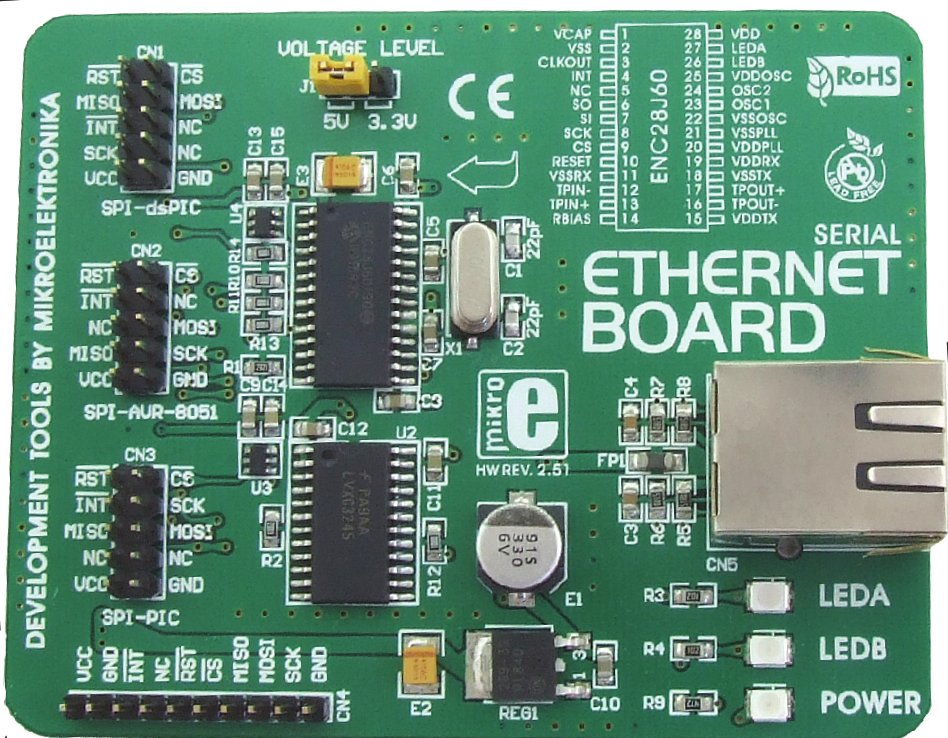
\includegraphics[width=.5\columnwidth]{pics/Ethernetboard.png}}
  \caption{Ethernet Board}
  \label{fig:ethernetboard}
\end{figure}

This extension board, as shown in figure \ref{fig:ethernetboard}, can be used for sending and receiving IEEE802.3 frames, and therefore embedding the developmentboard into a network. The board features an ethernet controller ENC28J60 that exchanges data with a microcontroller via standard SPI. The board can be connected to dsPIC, AVR-8051 and PIC by three 10-pin IDC connectors. The board needs 3.3V voltage supply, but has a 74LVXc3245 bus transceiver chip for running the board with 5V logic levels. Therefore, jumper J1 has to be set correctly.

A basic udp/ip/arp - stack has been implemented, with the following limitations:

\begin{itemize}
 \item No UDP - level checksum
 \item No IP - level options
 \item No IP - level fragmentation
 \item ARP request/reply only
 \item No ICMP
\end{itemize}

For using the extensionboard with the bigAVR6, the following requirements have to be provided:

\begin{itemize}
 \item Jumper J1 on the Ethernetboard must be set to 5V
 \item SPI-AVR-8051 VCC  must be connected to 5V
 \item SPI-AVR-8051 GND  must be connected to ground
 \item SPI-AVR-8051 CS   must be connected to PORT B0
 \item SPI-AVR-8051 SCK  must be connected to PORT B1
 \item SPI-AVR-8051 MOSI must be connected to PORT B2
 \item SPI-AVR-8051 MISO must be connected to PORT B3
 \item SPI-AVR-8051 RST  must be connected to PORT B4
 \item SPI-AVR-8051 INT  must be connected to PORT D2  
\end{itemize}

Obviously, the state of this connected pins \textbf{MUST NOT} be touched by the programmer.

To use the UDP - stack in an application, component UDPC with interface UDP has to be used. Interface UDP provides functions for initializing the stack and sending and receiving frames, as shown in listing \ref{UDP}.

\lstinputlisting[caption={UDP.nc},label=UDP]{../tinyos/tos/platforms/bigAVR6/udp/UDP.nc}


When the application wants to send data to or receive from a remote host, it initializes the stack by calling

\begin{lstlisting}
  command uint8_t initStack();
\end{lstlisting}

To send data, the corresponding function must be called:

\begin{lstlisting}
  command uint8_t sendData(uint16_t *dataPtr, uint8_t *destPtr, uint16_t srcPort,
			   uint16_t destPort, uint16_t len);
\end{lstlisting}

Afterwards, the data travels down the stack, as shown in figure \ref{fig:udpstack}. At first, an udp header is generated, and the payload, as assigned by the application, is attached to it. As mentioned above, \textbf{NO} checksum is generated at this level - if needed, a checksum must be calculated at application level. This udp packet(payload + udp-header) is then assigned to the next level, the ip level.

At this level, a checksum is generated, which includes the IP-header only. In the next step, a routing-decision has to be made: either the packet is addressed to a host \textit{inside} the lan(the remote host has the same network-adress than the ip that has been assigned to the bigAVR6 board), or the packet must \textit{hop} outside the lan. In the first case, the packet can be sent to the host directly, otherwise, it must be sent to the default gateway, as defined in the headerfile tinyos/tos/platforms/bigAVR6/ip/IP.h. When the proper destination ip has been found, an ARP - lookup is done. A local arp-cache is implemented as a ringbuffer, which saves ip/mac - address couples in a two-dimensional array. If no ARP - entry is found for the destionation ip, a lookup is sent automatically. Be aware that, if no MAC is found, the ARP-request - triggering packet is lost and must be resent by the application. If the MAC is known, it is extracted from the MAC cache, and component IEEE802.3 takes over control, where the frameheader and the payload(data + udp-header + ip-header) is copied into the transmit memory of the ENC28J60 by SPI. Afterwards, the communication is started, and the completion is signaled to the application.

To receive a packet from remote hosts, the packet must either has the proper destination MAC set, as defined in tinyos/tos/platforms/bigAVR6/eth/IEEE8023.h, or must be be a multicast frame(destination 0xFFFFFFFFFFFF), otherwise the ethernetcontroller chip ENC28J60 will not accept it. If a valid MAC is present, the ENC28J60 will autonomously copy the packet into the receive buffer and signal completion by an interrupt. The packet will be read out by component IEEE8023C and handed over to the IP-level component IPC. If the packet is a ARP - request, a corresponding reply will be sent, otherwise the payload(data + udp-header) will be handed over one level higher, which is the UDP - level. Note that the ip-checksum will \textbf{NOT} be checked. At UPD level, the actual payload will get extracted and is handed over to the application.

\begin{figure}[h]
 \centerline{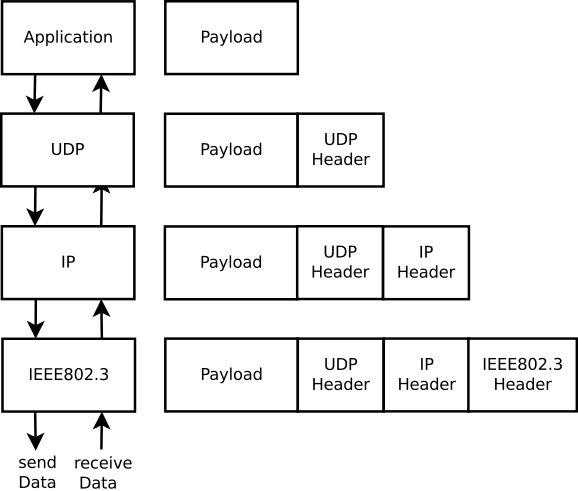
\includegraphics[width=.8\columnwidth]{pics/udpstack.png}}
  \caption{UPD Stack}
  \label{fig:udpstack}
\end{figure}

\subsection{LCD 2x16}



%%
%% = eof =====================================================================
%%
